\chapter{針對不同使用情境最佳化組態與朗博次方}
\label{chp:5}


\section{簡介}

此章節要針對特定情境進行最佳化,希望針對該情境,藉由調整LED與PD的硬體參數以及擺放位置,改善系統的量測表現,流程圖如\ref{flow:opt}。

\begin{figure}[ht]
    \centering
    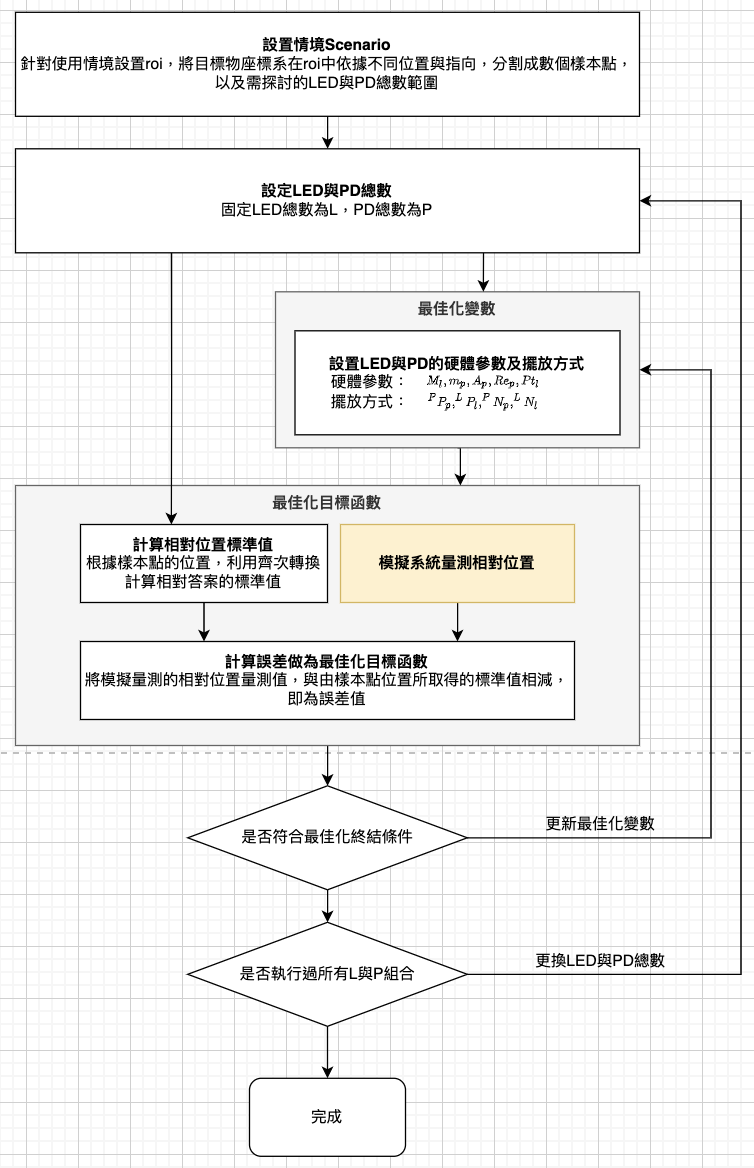
\includegraphics[width=13cm]{ch4pic/flowchart_opt.png}
    \caption{最佳化流程圖}
    \label{flow:opt}
\end{figure}

\clearpage

\subsection{情境設定}

需先定義此量測工況中觀察者座標系的ROI(Region of Interest),擁有此資訊後,將此範圍切割成數個樣本點位置(圖\ref{pic:testpoint})。我們將觀察者的PD座標系固定,將目標物的LED座標系放置於各樣本點,所有樣本點的平均誤差即為量測表現,誤差愈小代表量測表現愈好。

\begin{figure}[ht]
    \centering
    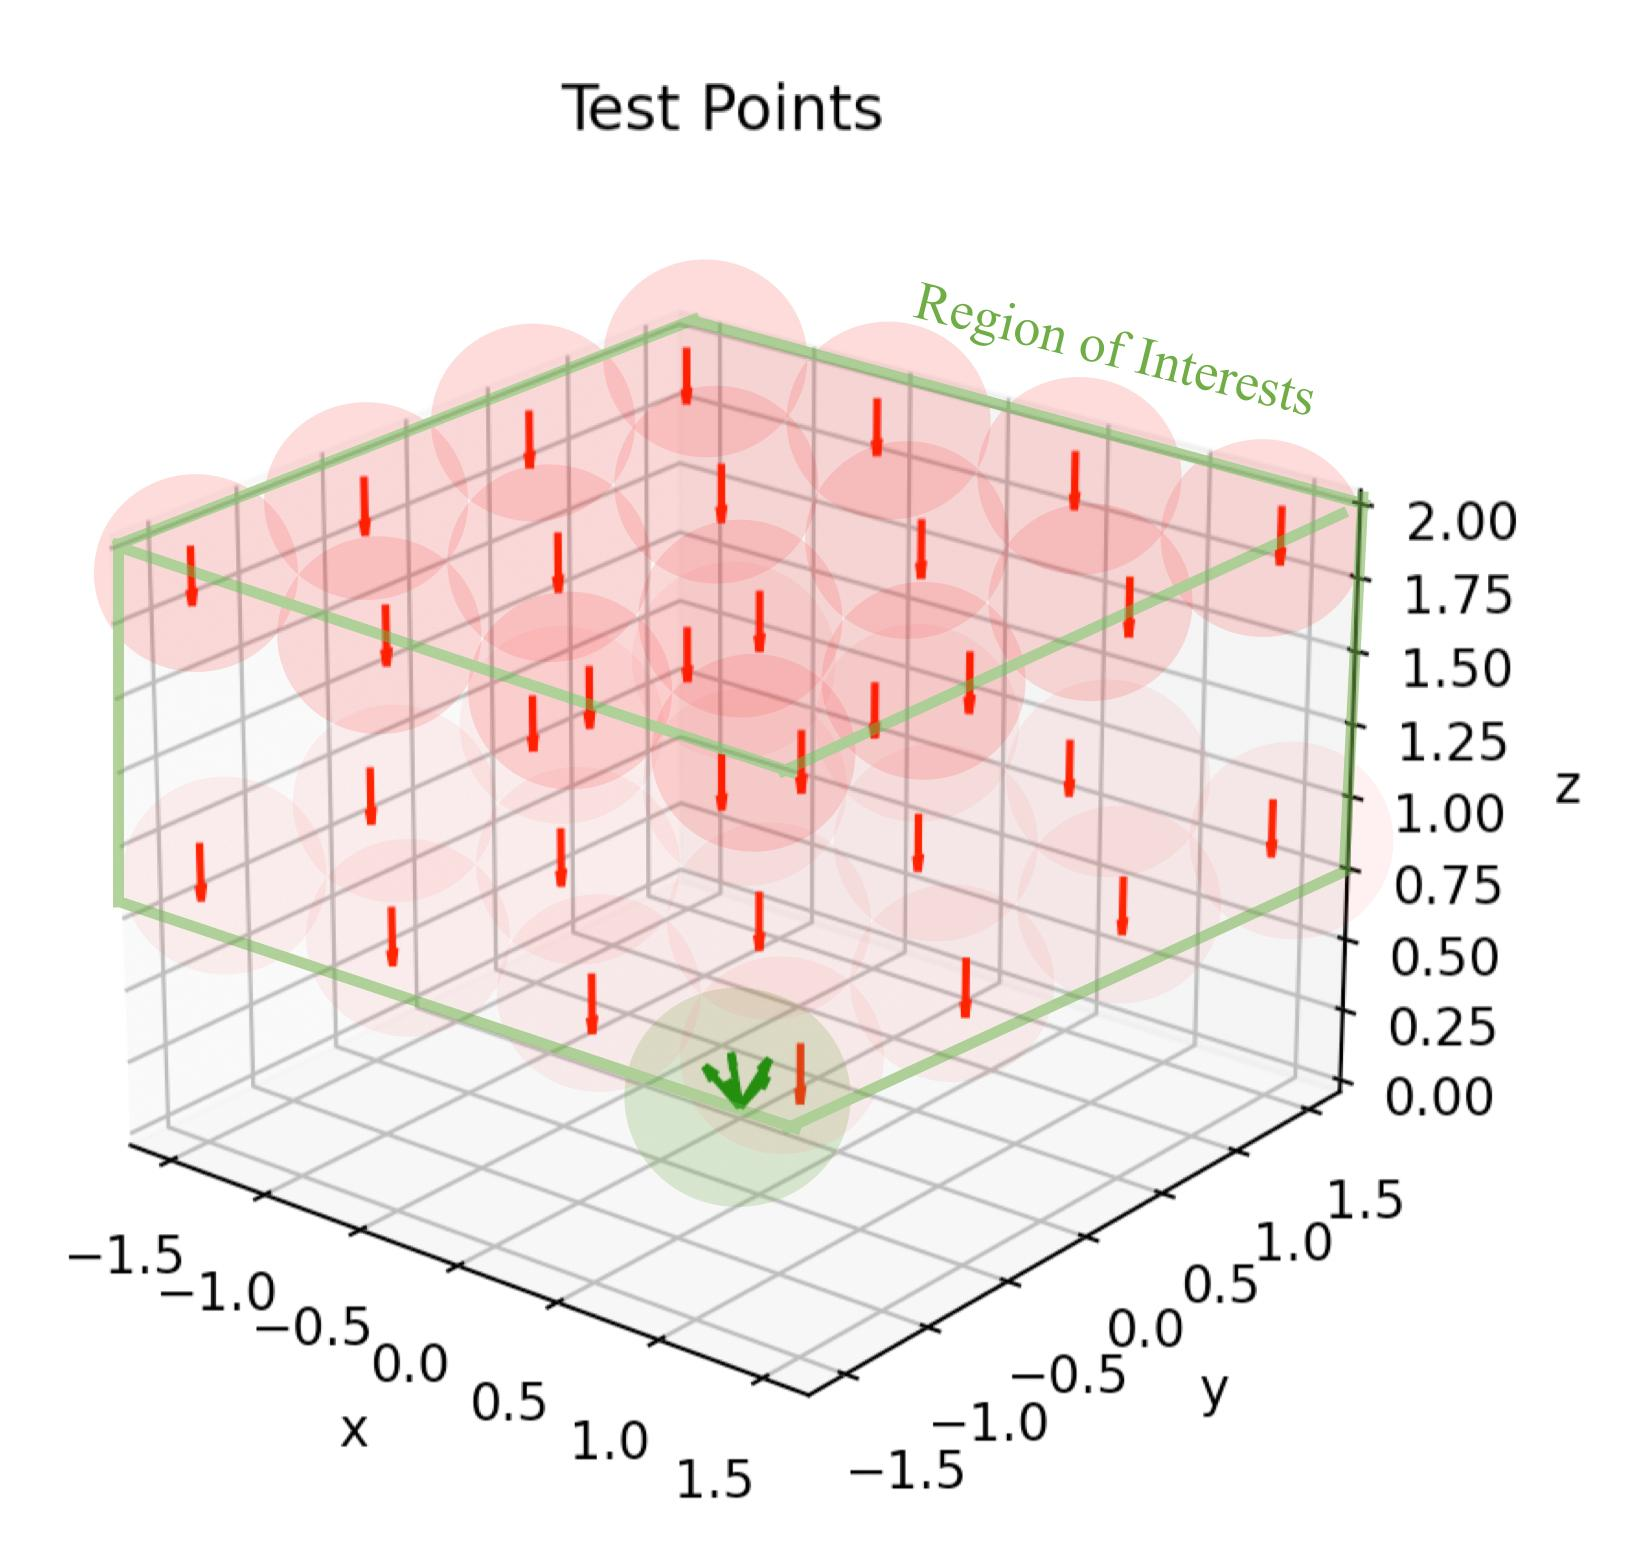
\includegraphics[width=8cm]{ch3pic/testpoint.jpg}
    \caption{ROI與樣本點示意圖}
    \label{pic:testpoint}
\end{figure}

\clearpage

\subsection{目標函數}

愈改善之目標為系統表現,期望能降低系統在ROI中的平均量測誤差,因此由\ref{eqn:objective}表示,將$K$個樣本點中的模擬量測相對位置與標準相對位置相減後,總和除$K$則得平均誤差;其中標準相對位置,為各樣本點相對PD座標系的位置;而模擬量測位置則利用第三章的方式進行數據處理所得。


(參考\ref{flow:opt})

\begin{figure}[ht]
    \centering
    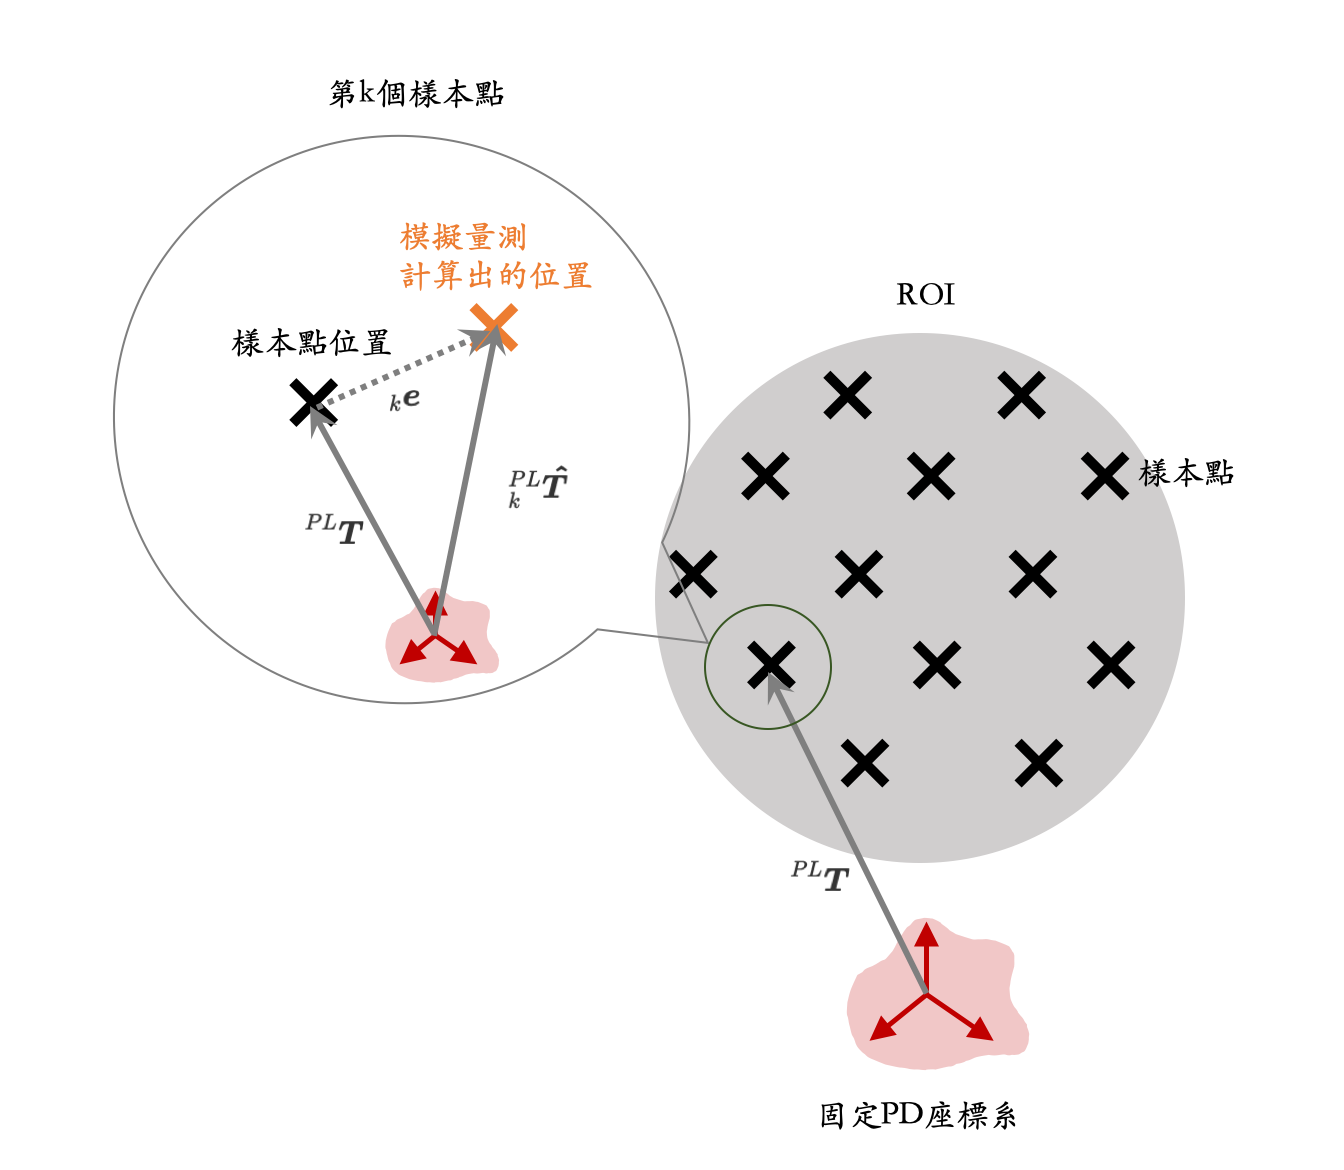
\includegraphics[width=8cm]{ch4pic/error.png}
    \caption{誤差示意圖}
    \label{pic:error}
\end{figure}


\begin{equation}
    \label{eqn:objective}
    \underset{^{P}P_p, ^{L}P_l,^{P}N_p, ^{L}N_l,Ml_l,Mp_p,A_p,Re_p,Pt_l}{\operatorname{minimize}} 
    \quad f = 
    \frac{\sum_{i=1}^{K}(||^{PL}_k\boldsymbol{T} -\hat{^{PL}_k\boldsymbol{T} } ||)}{K}  \\
\end{equation}


\begin{align*} \text{where }
    &p=1,2,...,P\\&l=1,2,...,L
\end{align*}



\subsection{最佳化變數}

硬體參數:$M_l,m_p,A_p,Re_p,Pt_l$

擺設方式:$^{P}P_p, ^{L}P_l,^{P}N_p, ^{L}N_l$

\begin{figure}[ht]
    \centering
    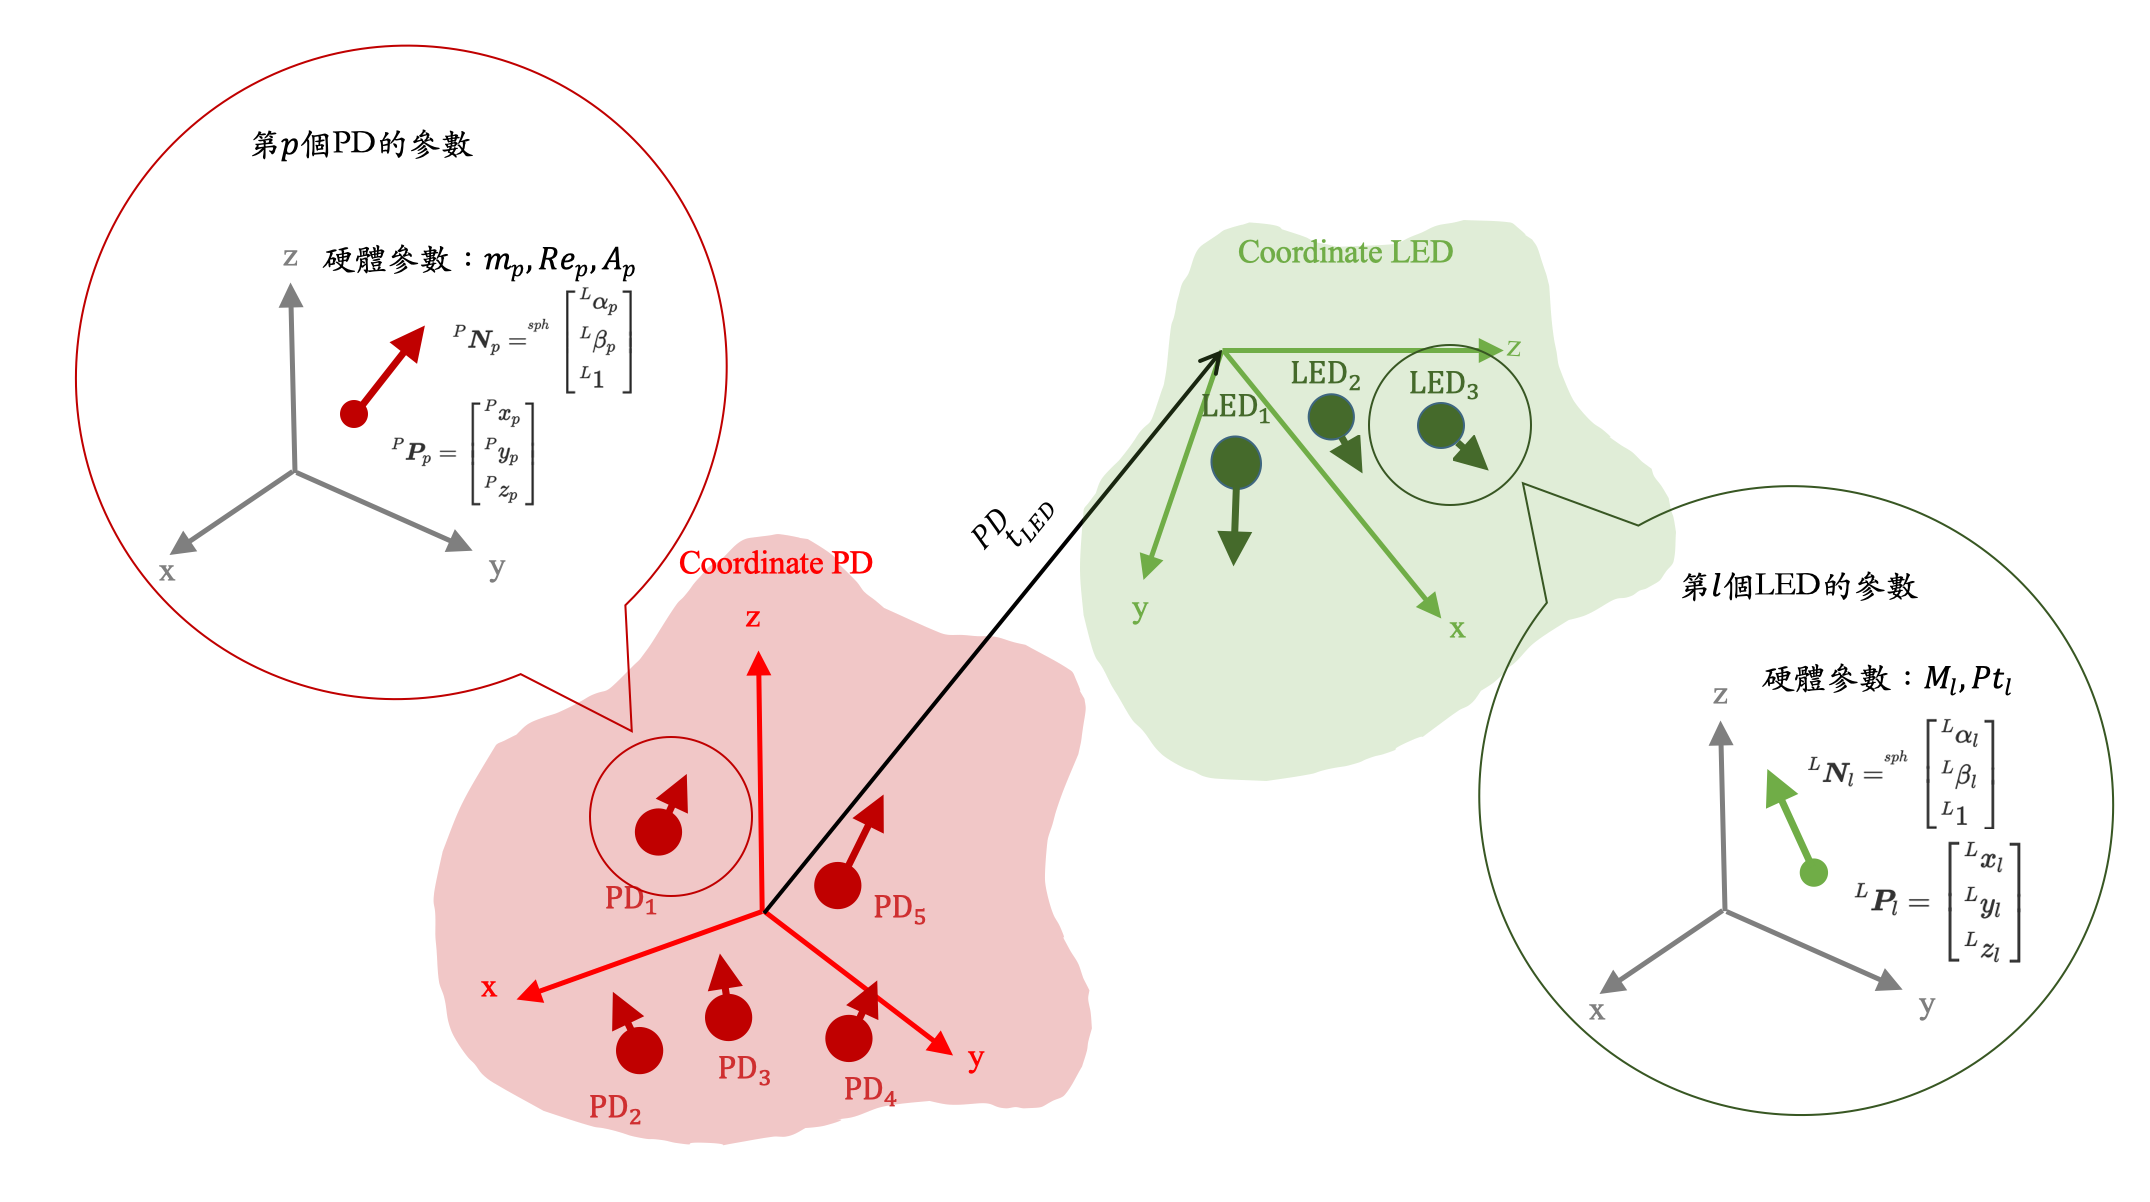
\includegraphics[width=12cm]{ch4pic/variable.png}
    \caption{最佳化變數}
    \label{pic:variable}
\end{figure}